\documentclass{standalone}

\usepackage[latin1]{inputenc}
\usepackage{tikz}
\usetikzlibrary{shapes,arrows}

\usepackage{bm}

\definecolor{policycolor}{rgb}{0.05, 0.45, 0.05}
\definecolor{modelcolor}{rgb}{0.9, 0.18, 0.0}
\definecolor{disscolor}{rgb}{0.9, 0.75, 0.15}
\definecolor{blueA}{rgb}{0.0,0.25,0.9}
\definecolor{crimson}{rgb}{0.86, 0.08, 0.24}

\tikzset{every picture/.style={/utils/exec={\sffamily}}}
\usetikzlibrary{shapes,arrows,positioning,automata,calc}

\begin{document}
\pagestyle{empty}


% Define block styles
%\tikzstyle{decision} = [diamond, draw, fill=blue!20, 
%    text width=4.5em, text badly centered, node distance=3cm, inner sep=0pt]
%\tikzstyle{block} = [rectangle, draw, text width=10em, text centered, rounded corners, minimum height=4em]
%\tikzstyle{line} = [draw, -latex']
%\tikzstyle{cloud} = [draw, ellipse,fill=red!20, node distance=3cm,
%    minimum height=2em]
    
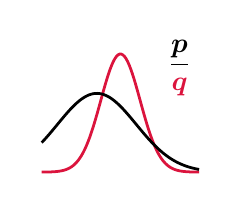
\begin{tikzpicture}[node distance = 1.5cm, auto, >=latex,
   action/.style={draw,thick},
   test/.style={draw, thick, shape aspect=2.7, diamond},
   every text node part/.style={align=center}]
   
    \node [transparent, rectangle, draw, text width=6em, text centered, rounded corners, minimum height=
    6em, color=black, align=left] (pi) {};
    
    %$\qquad\qquad \pi_{\bm{\theta}}$ \\ $ $ \\ $ $ \\ $ $  
	%\draw ($(pi) + (-0.4,0.7)$) node[color=blue!30!black] (a) {$\pi_{\bm{\theta}}$};    
    %\draw ($(pi) + (+0.7,0.3)$) node[color=blue!50] (a) {$\pi_{\bm{\theta}'}$}; 
    \draw ($(pi) + (0.75,0.55)$) node (a) {$\displaystyle \frac{\textcolor{black}{\bm{p}}}{\textcolor{crimson}{\bm{q}}}$};
    
	\def\normal{\x,{1.5*exp(-8*(\x)^2)}};
	\draw [color=crimson, domain=-1:1, samples=100, line width=1pt,yshift=-22] plot (\normal);
	
	\def\normali{\x,{1*exp(-2*(\x + .3)^2)}};
	\draw [color=black, domain=-1:1, samples=100, line width=1pt,yshift=-22] plot (\normali);
   	
   	
    % Place nodes
   
       
%    \node [cloud, left of=init] (expert) {expert};
%    \node [cloud, right of=init] (system) {system};
%    \node [block, below of=identify] (evaluate) {evaluate candidate models};
%    \node [block, left of=evaluate, node distance=3cm] (update) {update model};
%    \node [decision, below of=evaluate] (decide) {is best candidate better?};
%    \node [block, below of=decide, node distance=3cm] (stop) {stop};
    % Draw edges
    %\path [line] (init) |- (identify);
    %\draw ($(init) - (3.7,0)$) node {\footnotesize Agent $\footnotesize (\pi, \nu, Q^{\pi}, ...)$ \\ \vspace{-0.1cm}  \\ $\footnotesize \{\tau_i\}_{i=1}^N \sim $ \footnotesize Agent};
    %\draw[->, thick] (init) -- ($ (init) + (2.2,0) $);
   
    
    %\node[inner sep=0pt] (russell) at ($(identify.east) - (-0.7,0.7cm)$) {\includegraphics[scale=0.02]{style_img/brain_white}};
     %\node[inner sep=0pt] (russell) at ($(init.east) - (-0.3,0.7cm)$) {\includegraphics[scale=0.02]{style_img/brain_green}};
%    \begin{scope}[blend group=lighten];
%    \begin{scope}[blend group=difference]
%      \node[inner sep=0,line width=0] (logo) {\includegraphics{style_img/brain}};
%      \fill[black] (logo.south west) rectangle (logo.north east);
%    \end{scope}
%    \fill[orange] (logo.south west) rectangle (logo.north east);
%  \end{scope}
%    \path [line] (init) -- (identify);
%    \path [line] (identify) -- (evaluate);
%    \path [line] (evaluate) -- (decide);
%    \path [line] (decide) -| node [near start] {yes} (update);
%    \path [line] (update) |- (identify);
%    
%    \path [line] (decide) -- node {no}(stop);
%    \path [line,dashed] (expert) -- (init);
%    \path [line,dashed] (system) -- (init);
%    \path [line,dashed] (system) |- (evaluate);
\end{tikzpicture}


\end{document}